  \section{Marco Teórico}

    Una forma de obtener dicha respuesta, es generar un barrido en frecuencia 
    y registrar punto por punto, un esquema que se puede emplear para ello es el que 
    se observa en la Figura \ref{fig:GenBarrido}.
      \begin{figure}[H]
        \centering
          \frame{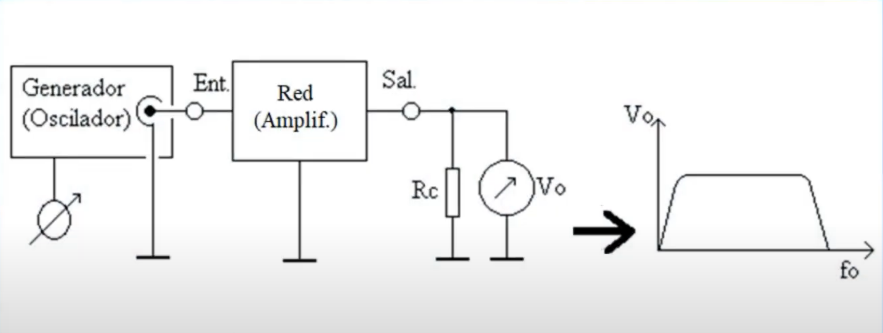
\includegraphics[width=0.6\textwidth]{Imagenes/ActividadPractica/MarcoTeorico/EsquemaGeneradorBarrido.png}}
          \caption{Esquema de barrido en frecuencia.}
          \label{fig:GenBarrido}
      \end{figure}

    Aunque el método propuesto es útil, en la práctica resulta complicado realizar el 
    registro de valores. Como solución al problema planteado, se puede utilizar un generador 
    de barrido el cual posee una salida modulada en frecuencia, ligada a una señal triangular,   
    que también está disponible como salida. Este dispositivo se puede utilizar en conjunto 
    con un osciloscopio, para simular el compartamiento de un analizador de redes, que 
    permite visualizar de forma automática la respuesta en frecuencia. 
    La Figura \ref{fig:GenBarridoRed} muestra un posible esquema de conexión. 

      \begin{figure}[H]
        \centering
          \frame{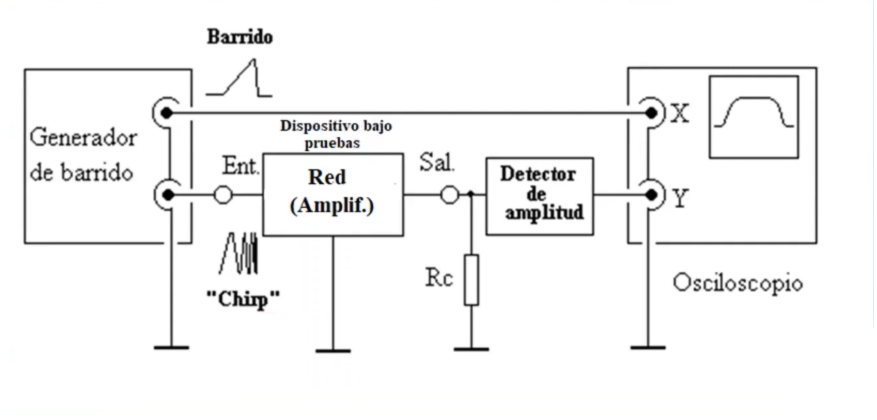
\includegraphics[width=0.6\textwidth]{Imagenes/ActividadPractica/MarcoTeorico/EsquemaGeneradorBarridoYRed.png}}
          \caption{Análisis de red usando un generador de barrido.}
          \label{fig:GenBarridoRed}
      \end{figure}
    
    Con esta segunda alternativa presentada, se logra obtener la respuesta en frecuencia de 
    una red bajo análisis. Sin embargo, no es posible conocer, con exactitud, la frecuencia 
    a la cual pertenece cada medición. Por ésta razón, se hace uso de un generador de marcas.
    La Figura~\ref{fig:GenBarridoYMarca} muestra un generador de barrido y de marcas en 
    conjunto. 
      \begin{figure}[H]
        \centering
          \frame{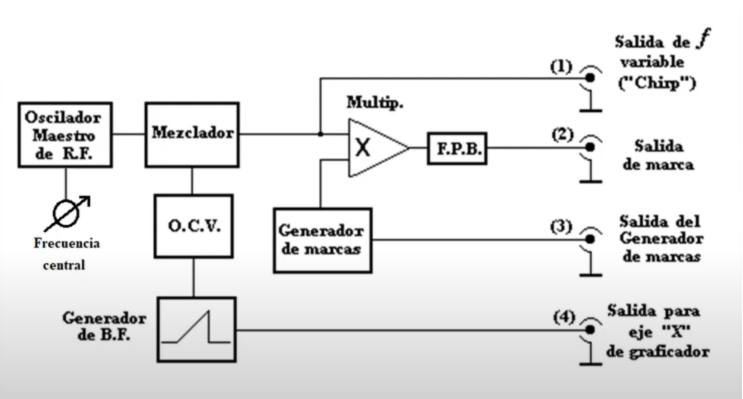
\includegraphics[width=0.6\textwidth]{Imagenes/ActividadPractica/MarcoTeorico/EsquemaGeneradorDeBarridoYMarcas.png}}
          \caption{Esquema de generador de barrido y marcas.}
          \label{fig:GenBarridoYMarca}
      \end{figure}

    La salida de marca proviene de un modulador en conjunto con un filtro pasa bajos 
    (generada con el método del batido cero), que se conoce como \textit{PIP}.
    Dicha señal se suma a la respuesta de la red bajo análisis, y se obtiene la salida 
    del canal vertical. De esta forma, la marca permite determinar la frecuencia. En la 
    Figura~\ref{fig:GenBarridoYMarcaOscilos} se muestra el esquema del análisis de una 
    red con un osciloscopio y un generador de barrido y marcas. 
      \begin{figure}[H]
        \centering
          \frame{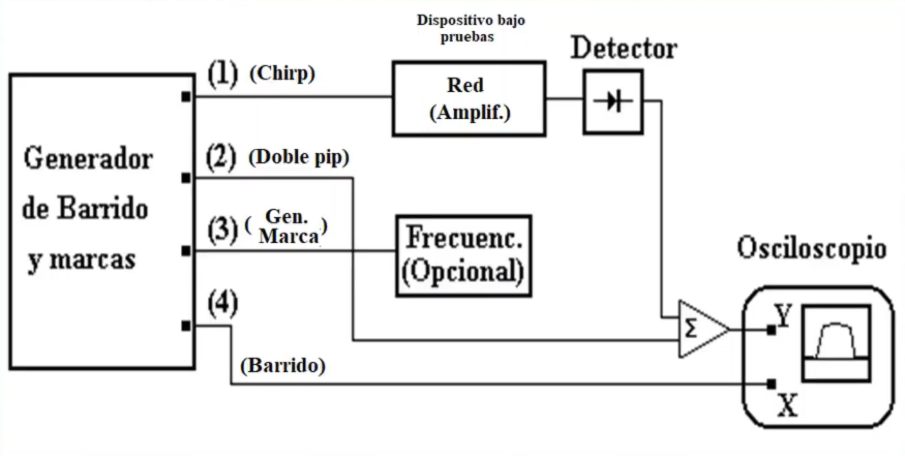
\includegraphics[width=0.6\textwidth]{Imagenes/ActividadPractica/MarcoTeorico/EsquemaGeneradorDeBarridoYMarcasOsciloscopio.png}}
          \caption{Esquema de osciloscopio y generador de barrido y marcas.}
          \label{fig:GenBarridoYMarcaOscilos}
      \end{figure}


    Los ensayos se pueden realizar en un receptor FM, cuyo esquema simplificado se presenta 
    en la Figura \ref{fig:ReceptorSimplificado}.
      \begin{figure}[H]
        \centering
          \frame{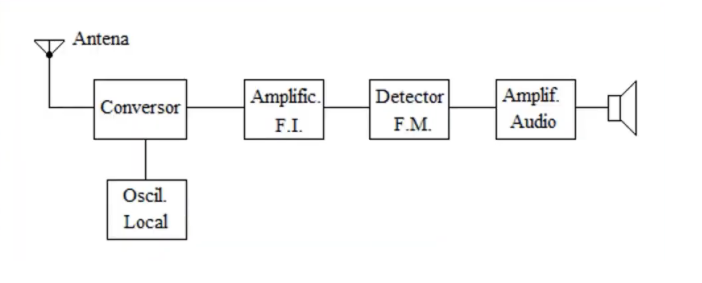
\includegraphics[width=0.6\textwidth]{Imagenes/ActividadPractica/MarcoTeorico/EsquemaSimplificadoReceptorFM.png}}
          \caption{Esquema de Detector FM simplificado.}
          \label{fig:ReceptorSimplificado}
      \end{figure}

    Se considera como etapa amplificadora, al conjunto formado por el conversor 
    y el amplificador, que conforman lo que se denomina \textit{amplificador sintonizado}.

    La salida del amplificador se combina con el detector para dar la señal resultante. 
    Bajo éste análisis, se deduce la salida del receptor de FM, que muestra la 
    Figura \ref{fig:FdeTReceptor}. Dicha salida es de utilidad para realizar los ensayos 
    propuestos en el presente informe.

      \begin{figure}[H]
        \centering
          \frame{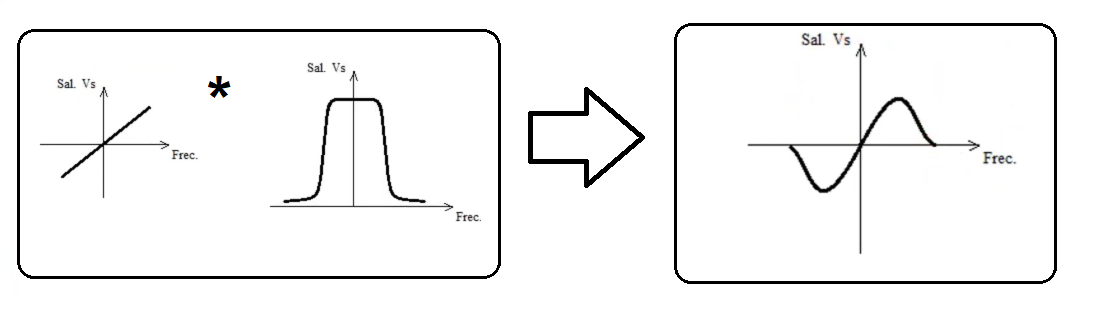
\includegraphics[width=0.6\textwidth]{Imagenes/ActividadPractica/MarcoTeorico/FdeTDetector.png}}
          \caption{Salida del detector.}
          \label{fig:FdeTReceptor}
      \end{figure}

